\documentclass[aspectratio=169]{beamer}

% --- Theme & Colors -----------------------------------------------------------
\usetheme{Madrid}
\usecolortheme{default}
\setbeamertemplate{navigation symbols}{}
\setbeamertemplate{footline}[frame number]

% --- Packages -----------------------------------------------------------------
\usepackage{amsmath,amssymb}
\usepackage{booktabs}
\usepackage{array}
\usepackage{xcolor}
\usepackage{tikz}
\usepackage{pgfplots}
\pgfplotsset{compat=1.18}
\usetikzlibrary{arrows.meta, positioning}

% --- Colors -------------------------------------------------------------------
\definecolor{qeblue}{RGB}{31,119,180}
\definecolor{qeorange}{RGB}{255,127,14}
\definecolor{qegreen}{RGB}{44,160,44}
\definecolor{qered}{RGB}{214,39,40}
\setbeamercolor{structure}{fg=qeblue}

% --- Macros -------------------------------------------------------------------
\newcommand{\E}{\mathbb{E}}
\newcommand{\R}{\mathbb{R}}
\newcommand{\pbar}{\bar{p}}
\newcommand{\pcheck}{\check{p}}
\newcommand{\pha}{\hat{p}_a}
\newcommand{\phb}{\hat{p}_b}
\newcommand{\Pa}{P_a}
\newcommand{\Pb}{P_b}

% --- Title --------------------------------------------------------------------
\title[Heterogeneous Beliefs \& Bubbles]{Heterogeneous Beliefs and Bubbles}
\subtitle{Harrison--Kreps (1978) --- QuantEcon Lecture 89}
\author{Thomas J.\ Sargent \and John Stachurski}
\institute{QuantEcon}
\date{March 2026}

% ==============================================================================
\begin{document}
% ==============================================================================

\begin{frame}
  \titlepage
\end{frame}

% ------------------------------------------------------------------------------
\begin{frame}{Outline}
  \tableofcontents
\end{frame}

% ==============================================================================
\section{Overview}
% ==============================================================================

\begin{frame}{Overview}
  \begin{block}{The Harrison--Kreps Model}
    Determines the \textbf{equilibrium price} of a dividend-yielding asset
    traded by two types of self-interested investors.
  \end{block}

  \medskip
  The model features:
  \begin{itemize}
    \item Heterogeneous beliefs about dividends
    \item Incomplete markets
    \item Short-sales constraints
    \item (Possibly) leverage limits on borrowing to finance asset purchases
  \end{itemize}

  \medskip
  \begin{block}{Reference}
    Harrison, J.~M.\ and Kreps, D.~M.\ (1978).
    ``Speculative Investor Behavior in a Stock Market with Heterogeneous
    Expectations.''
    \emph{Quarterly Journal of Economics}, 92(2), 323--336.
  \end{block}
\end{frame}

% ------------------------------------------------------------------------------
\begin{frame}{What Is a Bubble?}
  Economists differ on definitions. The Harrison--Kreps model illustrates:

  \bigskip
  \begin{alertblock}{A Working Definition of a Bubble}
    A component of an asset price can be interpreted as a \textbf{bubble} when
    \emph{all} investors agree that the current price of the asset exceeds what
    they believe the asset's underlying dividend stream justifies.
  \end{alertblock}

  \bigskip
  We will see that this can arise in equilibrium when
  \begin{enumerate}
    \item Investors have \emph{heterogeneous} beliefs, and
    \item Short sales are \emph{prohibited} (pessimists cannot short).
  \end{enumerate}
\end{frame}

% ==============================================================================
\section{Structure of the Model}
% ==============================================================================

\begin{frame}{Asset and Dividends}
  \begin{columns}
    \column{0.55\textwidth}
    \begin{itemize}
      \item Fixed supply of $A$ shares of a risky asset.
      \item Dividends $\{d_t\}$ follow a \textbf{two-state Markov chain}:
        \[
          S = \{0,1\}, \qquad
          d_t = \begin{cases} 0 & s_t = 0 \\ 1 & s_t = 1 \end{cases}
        \]
      \item Stock is traded \textbf{ex dividend}: owning a share at end of $t$
        entitles the holder to the dividend at $t+1$ and the right to sell at
        $t+1$.
    \end{itemize}

    \column{0.42\textwidth}
    \begin{center}
    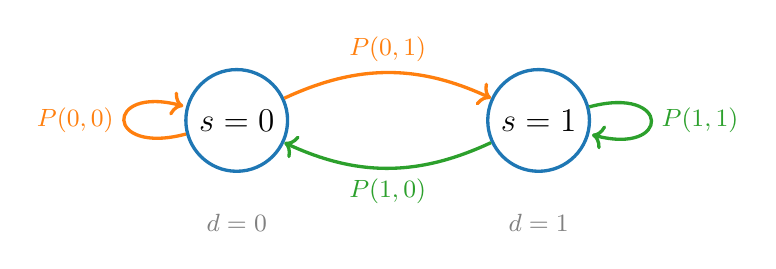
\begin{tikzpicture}[
        node distance=2.5cm,
        state/.style={circle, draw=qeblue, very thick, minimum size=1.2cm,
                      font=\large\bfseries}
      ]
      \node[state] (s0) {$s=0$};
      \node[state] (s1) [right=of s0] {$s=1$};

      \draw[->, very thick, qeorange]
        (s0) edge[bend left=25] node[above]{\small $P(0,1)$} (s1);
      \draw[->, very thick, qegreen]
        (s1) edge[bend left=25] node[below]{\small $P(1,0)$} (s0);
      \draw[->, very thick, qeorange]
        (s0) edge[loop left] node{\small $P(0,0)$} (s0);
      \draw[->, very thick, qegreen]
        (s1) edge[loop right] node{\small $P(1,1)$} (s1);

      \node[below=0.4cm of s0, font=\small\color{gray}] {$d=0$};
      \node[below=0.4cm of s1, font=\small\color{gray}] {$d=1$};
    \end{tikzpicture}
    \end{center}
  \end{columns}
\end{frame}

% ------------------------------------------------------------------------------
\begin{frame}{Two Types of Investors}
  Two types $h \in \{a,b\}$ of risk-neutral investors share a \textbf{common
  discount factor} $\beta = 0.75$ but hold \textbf{different beliefs} about
  the Markov transition matrix, $P(i,j) = \Pr\{s_{t+1}=j \mid s_t=i\}$:

  \bigskip
  \begin{columns}
    \column{0.48\textwidth}
    \begin{block}{Type $a$ believes}
      \[
        \Pa =
        \begin{bmatrix}
          \tfrac{1}{2} & \tfrac{1}{2} \\[4pt]
          \tfrac{2}{3} & \tfrac{1}{3}
        \end{bmatrix}
      \]
    \end{block}

    \column{0.48\textwidth}
    \begin{block}{Type $b$ believes}
      \[
        \Pb =
        \begin{bmatrix}
          \tfrac{2}{3} & \tfrac{1}{3} \\[4pt]
          \tfrac{1}{4} & \tfrac{3}{4}
        \end{bmatrix}
      \]
    \end{block}
  \end{columns}

  \bigskip
  \begin{itemize}
    \item In state $0$: type $a$ is \textcolor{qegreen}{\textbf{more optimistic}}
          about tomorrow's dividend than type $b$
          \quad $[\tfrac{1}{2} > \tfrac{1}{3}]$
    \item In state $1$: type $b$ is \textcolor{qegreen}{\textbf{more optimistic}}
          about tomorrow's dividend than type $a$
          \quad $[\tfrac{3}{4} > \tfrac{1}{3}]$
  \end{itemize}
\end{frame}

% ------------------------------------------------------------------------------
\begin{frame}{Stationary Distributions}
  The \textbf{long-run} (stationary) distributions of the two transition
  matrices are:

  \bigskip
  \begin{columns}
    \column{0.48\textwidth}
    \begin{block}{Type $a$: stationary distribution}
      \[
        \pi_a \approx \begin{bmatrix} 0.571 & 0.429 \end{bmatrix}
      \]
      Type $a$ spends more time in the \emph{low-dividend} state.\\[4pt]
      $\Rightarrow$ \textbf{more pessimistic on average}.
    \end{block}

    \column{0.48\textwidth}
    \begin{block}{Type $b$: stationary distribution}
      \[
        \pi_b \approx \begin{bmatrix} 0.429 & 0.571 \end{bmatrix}
      \]
      Type $b$ spends more time in the \emph{high-dividend} state.\\[4pt]
      $\Rightarrow$ \textbf{more optimistic on average}.
    \end{block}
  \end{columns}

  \bigskip
  \begin{alertblock}{Key insight}
    Beliefs are \emph{stochastically alternating}: each type is temporarily
    optimistic in one state and temporarily pessimistic in the other.
  \end{alertblock}
\end{frame}

% ------------------------------------------------------------------------------
\begin{frame}{Ownership Rights, Short Sales, and Leverage}
  \begin{block}{Ownership Rights}
    \begin{itemize}
      \item Owning a share at end of $t$ $\Rightarrow$ dividend at $t+1$ and
            right to sell at $t+1$.
      \item Both types are \textbf{risk-neutral}; common discount factor
            $\beta=0.75$.
    \end{itemize}
  \end{block}

  \medskip
  \begin{block}{No Short Sales}
    \begin{itemize}
      \item Pessimists \textbf{can} express their views by selling their shares.
      \item Pessimists \textbf{cannot} manufacture more shares by borrowing from
            optimists and immediately selling (no short selling).
    \end{itemize}
  \end{block}

  \medskip
  \begin{block}{Two Regimes to Study}
    \begin{enumerate}
      \item Each type has \emph{enough wealth} to purchase the entire stock
            (Harrison--Kreps's case).
      \item Neither type alone can purchase the entire stock---both must hold
            some shares.
    \end{enumerate}
  \end{block}
\end{frame}

% ------------------------------------------------------------------------------
\begin{frame}{Information}
  \begin{itemize}
    \item Investors know the current state $s_t$ when they decide to buy or
          sell.
    \item They also know a \textbf{price function}
          \[
            p: S \to \R_{+}, \quad s \mapsto p(s),
          \]
          which maps today's state into the equilibrium price.
    \item The price function is \emph{endogenous}---it must be determined in
          equilibrium.
  \end{itemize}
\end{frame}

% ==============================================================================
\section{Equilibrium Prices}
% ==============================================================================

\begin{frame}{Summary of Equilibrium Prices}
  \begin{center}
  \renewcommand{\arraystretch}{1.4}
  \begin{tabular}{lcc}
    \toprule
    \textbf{Scenario} & \textbf{State 0} & \textbf{State 1} \\
    \midrule
    $p_a$ \;(homogeneous beliefs $\Pa$) & 1.33 & 1.22 \\
    $p_b$ \;(homogeneous beliefs $\Pb$) & 1.45 & 1.91 \\
    \midrule
    $p_o$ \;(optimistic marginal investor) & \textbf{1.85} & \textbf{2.08} \\
    $p_p$ \;(pessimistic marginal investor) & 1.00 & 1.00 \\
    \midrule
    $\pha$ \;(willingness to pay, type $a$) & 1.85 & 1.69 \\
    $\phb$ \;(willingness to pay, type $b$) & 1.69 & 2.08 \\
    \bottomrule
  \end{tabular}
  \end{center}

  \bigskip
  \footnotesize Parameters: $\beta = 0.75$; $P_a$, $P_b$ as specified.
\end{frame}

% ------------------------------------------------------------------------------
\begin{frame}{Single Belief (Homogeneous) Pricing}
  When all investors are of type $h$, the no-arbitrage pricing equation is:
  \[
    p_h(s) = \beta \bigl[ P_h(s,0)\,(0 + p_h(0)) + P_h(s,1)\,(1 + p_h(1)) \bigr],
    \quad s=0,1.
  \]

  In vector form:
  \[
    \begin{bmatrix} p_h(0) \\ p_h(1) \end{bmatrix}
    = \beta\,[I - \beta P_h]^{-1} P_h \begin{bmatrix} 0 \\ 1 \end{bmatrix}
  \]

  \medskip
  \begin{columns}
    \column{0.48\textwidth}
    \begin{block}{Under $\Pa$}
      \[
        p_a(0) = 1.33, \quad p_a(1) = 1.22
      \]
    \end{block}
    \column{0.48\textwidth}
    \begin{block}{Under $\Pb$}
      \[
        p_b(0) = 1.45, \quad p_b(1) = 1.91
      \]
    \end{block}
  \end{columns}

  \medskip
  These are the \textbf{fundamental values} as each type perceives them---the
  expected discounted present value of future dividends under that type's
  beliefs.
\end{frame}

% ------------------------------------------------------------------------------
\begin{frame}{Pricing with Heterogeneous Beliefs: Optimistic Marginal Investor}
  \textbf{Case:} Both types have enough wealth to buy the entire stock; no
  short sales.

  \medskip
  The marginal investor who \emph{prices} the asset is the \textbf{temporarily
  optimistic} type. The equilibrium price $\pbar$ satisfies:

  \begin{alertblock}{Harrison--Kreps Key Equation}
    \[
      \pbar(s) = \beta \max\bigl\{
        P_a(s,\cdot)\cdot[\pbar + d],\;
        P_b(s,\cdot)\cdot[\pbar + d]
      \bigr\}, \quad s=0,1,
    \]
    where $d = \bigl[\begin{smallmatrix}0\\1\end{smallmatrix}\bigr]$
    and $P_h(s,\cdot)\cdot[\pbar+d]
       = P_h(s,0)\,\pbar(0) + P_h(s,1)\,(1+\pbar(1))$.
  \end{alertblock}

  \medskip
  \begin{itemize}
    \item The $\max$ selects whichever type values the asset more highly
          \emph{next period}.
    \item Type $a$ prices in state 0; type $b$ prices in state 1.
  \end{itemize}
\end{frame}

% ------------------------------------------------------------------------------
\begin{frame}{Solving the Functional Equation: Value Iteration}
  Like a Bellman equation, iterate to convergence:
  \[
    \pbar^{j+1}(s) = \beta \max\bigl\{
      P_a(s,0)\,\pbar^j(0) + P_a(s,1)\,(1+\pbar^j(1)),\;
      P_b(s,0)\,\pbar^j(0) + P_b(s,1)\,(1+\pbar^j(1))
    \bigr\}
  \]
  starting from any initial guess, e.g.\ $\pbar^0=(0,0)$.

  \medskip
  This operator is a \textbf{contraction mapping} $\Rightarrow$ unique fixed
  point.

  \medskip
  \begin{block}{Optimistic equilibrium prices}
    \[
      p_o(0) = 1.85, \qquad p_o(1) = 2.08.
    \]
    \textbf{Both exceed} $p_a(s)$ and $p_b(s)$ in every state!
  \end{block}
\end{frame}

% ------------------------------------------------------------------------------
\begin{frame}{Why Does the Bubble Arise?}
  Each investor's \textbf{willingness to pay} (holding value):

  \begin{columns}
    \column{0.48\textwidth}
    \begin{block}{Type $a$}
      \[
        \pha(s) = \begin{cases}
          \pbar(0) & s=0 \\[4pt]
          \beta\bigl[P_a(1,0)\,\pbar(0) \\
          \quad + P_a(1,1)(1+\pbar(1))\bigr] & s=1
        \end{cases}
      \]
      $\pha(0)=1.85,\quad \pha(1)=1.69$
    \end{block}

    \column{0.48\textwidth}
    \begin{block}{Type $b$}
      \[
        \phb(s) = \begin{cases}
          \beta\bigl[P_b(0,0)\,\pbar(0) \\
          \quad + P_b(0,1)(1+\pbar(1))\bigr] & s=0 \\[4pt]
          \pbar(1) & s=1
        \end{cases}
      \]
      $\phb(0)=1.69,\quad \phb(1)=2.08$
    \end{block}

  \end{columns}

  \medskip
  Note: $\pha(1)=1.69 < \pbar(1)=2.08$ and $\phb(0)=1.69 < \pbar(0)=1.85$.

  \begin{alertblock}{The resale-option premium}
    Each investor pays \emph{more} than their own fundamental value because they
    expect to resell to a more optimistic buyer later.
  \end{alertblock}
\end{frame}

% ------------------------------------------------------------------------------
\begin{frame}{Asset Trading Dynamics}

  \begin{center}
  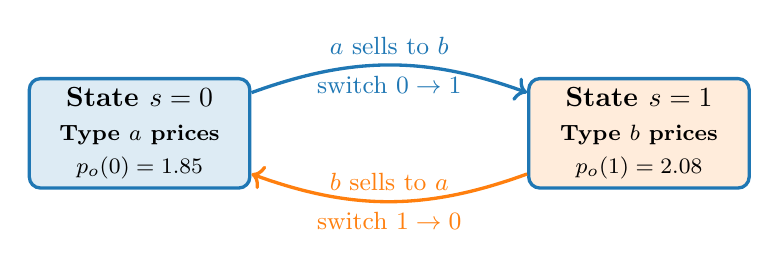
\begin{tikzpicture}[
      node distance=3.5cm,
      state/.style={rectangle, rounded corners, draw=qeblue, very thick,
                    minimum width=2.8cm, minimum height=1.2cm, align=center,
                    font=\bfseries}
    ]
    \node[state, fill=qeblue!15] (s0)
      {State $s=0$\\ \footnotesize Type $a$ prices\\ \footnotesize $p_o(0)=1.85$};
    \node[state, fill=qeorange!15] (s1) [right=of s0]
      {State $s=1$\\ \footnotesize Type $b$ prices\\ \footnotesize $p_o(1)=2.08$};

    \draw[->, very thick, qeblue, bend left=20]
      (s0) to node[above, font=\small\color{qeblue}]
        {$a$ sells to $b$}
        node[below, font=\small\color{gray}] {switch $0\to 1$}
      (s1);
    \draw[->, very thick, qeorange, bend left=20]
      (s1) to node[above, font=\small\color{qeorange}]
        {$b$ sells to $a$}
        node[below, font=\small\color{gray}] {switch $1\to 0$}
      (s0);
  \end{tikzpicture}
  \end{center}

  \bigskip
  \begin{itemize}
    \item The asset \textbf{changes hands} every time the state switches.
    \item High trading volume is a signature feature of this bubble model.
    \item Even the \emph{pessimistic} type at each state acknowledges the price
          exceeds its own fundamental value---yet still holds the asset.
  \end{itemize}
\end{frame}

% ------------------------------------------------------------------------------
\begin{frame}{Visualizing the Price Premium}
  \begin{center}
  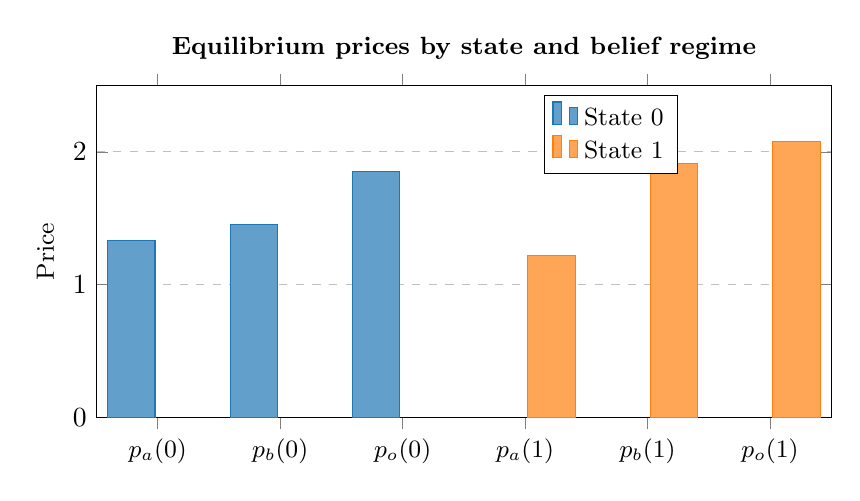
\begin{tikzpicture}
    \begin{axis}[
        ybar,
        bar width=0.6cm,
        width=0.9\linewidth, height=5.8cm,
        xtick={1,2,3,4,5,6},
        xticklabels={$p_a(0)$, $p_b(0)$, $p_o(0)$,
                     $p_a(1)$, $p_b(1)$, $p_o(1)$},
        xticklabel style={font=\small},
        ymin=0, ymax=2.5,
        ylabel={Price},
        ylabel style={font=\small},
        ymajorgrids=true,
        grid style=dashed,
        legend style={at={(0.7,0.97)}, anchor=north, font=\small},
        title={Equilibrium prices by state and belief regime},
        title style={font=\small\bfseries},
      ]
      % State 0 prices
      \addplot[fill=qeblue!70, draw=qeblue] coordinates {(1,1.33)(2,1.45)(3,1.85)};
      % State 1 prices
      \addplot[fill=qeorange!70, draw=qeorange] coordinates {(4,1.22)(5,1.91)(6,2.08)};
      \legend{State 0, State 1}
    \end{axis}
  \end{tikzpicture}
  \end{center}

  \footnotesize The optimistic equilibrium price $p_o$ exceeds both homogeneous
  belief benchmarks $p_a$ and $p_b$ in every state.
\end{frame}

% ------------------------------------------------------------------------------
\begin{frame}{Pricing with Pessimistic Marginal Investor: Insufficient Funds}
  \textbf{Case:} The optimistic type \emph{cannot} purchase the entire stock;
  both types must hold shares.  The asset price must attract pessimistic
  investors too.

  \begin{alertblock}{Pessimistic Pricing Equation}
    \[
      \pcheck(s) = \beta \min\bigl\{
        P_a(s,\cdot)\cdot[\pcheck + d],\;
        P_b(s,\cdot)\cdot[\pcheck + d]
      \bigr\}, \quad s=0,1.
    \]
  \end{alertblock}

  \medskip
  \begin{block}{Pessimistic equilibrium prices}
    \[
      p_p(0) = 1.00, \qquad p_p(1) = 1.00.
    \]
  \end{block}

  \medskip
  \begin{itemize}
    \item $p_p < p_a, p_b$ in every state---below both fundamental values.
    \item Optimistic investors think the asset is \emph{underpriced} but are
          prevented from leveraging up to buy more.
    \item Pessimistic pricing also arises if short sales \emph{are} allowed:
          pessimists short the asset until price falls to $\pcheck$.
  \end{itemize}
\end{frame}

% ==============================================================================
\section{Bubble Interpretation}
% ==============================================================================

\begin{frame}{Scheinkman's Interpretation}
  \begin{columns}
    \column{0.55\textwidth}
    \textbf{Jose Scheinkman (2014)} interprets Harrison--Kreps as a model of a
    bubble: an asset price that exceeds \emph{every} investor's estimate of
    fundamental value.

    \medskip
    Key predictions of the model:
    \begin{itemize}
      \item \textcolor{qegreen}{\textbf{High volume}} accompanies high
            (optimistic) prices---the asset changes hands with every state
            switch.
      \item Bubbles are supported by short-sales constraints and leverage.
      \item Bubbles \textbf{end} when asset supply grows enough to exceed
            optimistic investors' resources.
    \end{itemize}

    \column{0.42\textwidth}
    \begin{block}{Regulatory implications}
      \begin{itemize}
        \item \textbf{Limiting short sales} $\uparrow$ bubble prices
              (pessimists can't short).
        \item \textbf{Limiting leverage} $\downarrow$ bubble prices
              (optimists can't borrow to buy).
        \item These two regulations have \emph{opposite} effects!
      \end{itemize}
    \end{block}
  \end{columns}
\end{frame}

% ==============================================================================
\section{Extensions: Permanent Optimism and Pessimism}
% ==============================================================================

\begin{frame}{Permanently Optimistic and Pessimistic Investors}
  To interpret $p_o$ further, introduce two hypothetical special types:

  \bigskip
  \begin{columns}
    \column{0.48\textwidth}
    \begin{block}{Permanently optimistic investor}
      Holds the most optimistic view in \emph{each} state:
      \[
        P_{\mathrm{opt}} =
        \begin{bmatrix}
          \tfrac{1}{2} & \tfrac{1}{2} \\[4pt]
          \tfrac{1}{4} & \tfrac{3}{4}
        \end{bmatrix}
      \]
      (Takes the $\max$ column from $\Pa$ and $\Pb$ row by row.)
    \end{block}

    \column{0.48\textwidth}
    \begin{block}{Permanently pessimistic investor}
      Holds the least optimistic view in \emph{each} state:
      \[
        P_{\mathrm{pess}} =
        \begin{bmatrix}
          \tfrac{2}{3} & \tfrac{1}{3} \\[4pt]
          \tfrac{2}{3} & \tfrac{1}{3}
        \end{bmatrix}
      \]
      (Takes the $\min$ column from $\Pa$ and $\Pb$ row by row.)
    \end{block}
  \end{columns}

  \bigskip
  \begin{alertblock}{Key result}
    The equilibrium price under heterogeneous beliefs with optimistic marginal
    investor, $p_o$, \textbf{equals} the single-belief price of the
    \emph{permanently optimistic} investor.
  \end{alertblock}
\end{frame}

% ------------------------------------------------------------------------------
\begin{frame}{Extended Summary Table}
  \begin{center}
  \renewcommand{\arraystretch}{1.4}
  \begin{tabular}{lcc}
    \toprule
    \textbf{Scenario} & \textbf{State 0} & \textbf{State 1} \\
    \midrule
    $p_a$ \;(type $a$ only)         & 1.33 & 1.22 \\
    $p_b$ \;(type $b$ only)         & 1.45 & 1.91 \\
    $p_{\mathrm{opt}}$\;(perm.\ opt.)   & 1.85 & 2.08 \\
    $p_{\mathrm{pess}}$\;(perm.\ pess.) & 1.33 & 1.00 \\
    \midrule
    $p_o$ \;(optimistic marginal inv.)  & \textbf{1.85} & \textbf{2.08} \\
    $p_p$ \;(pessimistic marginal inv.) & 1.00 & 1.00 \\
    \midrule
    $\pha$ \;(type $a$ WTP)             & 1.85 & 1.69 \\
    $\phb$ \;(type $b$ WTP)             & 1.69 & 2.08 \\
    \bottomrule
  \end{tabular}
  \end{center}

  \smallskip
  \footnotesize $p_o = p_{\mathrm{opt}}$: the heterogeneous-beliefs equilibrium
  replicates the price of a permanently-optimistic single-belief market.
\end{frame}

% ==============================================================================
\section{Summary}
% ==============================================================================

\begin{frame}{Summary}
  \begin{enumerate}
    \item \textbf{Heterogeneous beliefs + no short sales = bubble.}
          Prices can exceed every investor's fundamental value.

    \medskip
    \item \textbf{The resale-option premium.} Investors overpay because they
          anticipate selling to a more optimistic buyer when the state changes.

    \medskip
    \item \textbf{Trading volume is high} along the bubble path---the asset
          changes hands every time the Markov state switches.

    \medskip
    \item \textbf{The optimistic equilibrium price equals the single-belief
          price of a permanently-optimistic investor.}

    \medskip
    \item \textbf{Regulatory asymmetry:} limiting short sales \emph{inflates}
          bubbles; limiting leverage \emph{deflates} them.

    \medskip
    \item \textbf{Supply matters:} expanding asset supply beyond optimists'
          financial capacity extinguishes the bubble.
  \end{enumerate}
\end{frame}

% ------------------------------------------------------------------------------
\begin{frame}{References}
  \begin{itemize}
    \item Harrison, J.~M.\ and Kreps, D.~M.\ (1978).
          ``Speculative Investor Behavior in a Stock Market with Heterogeneous
          Expectations.''
          \emph{Quarterly Journal of Economics}, \textbf{92}(2), 323--336.

    \medskip
    \item Scheinkman, J.~A.\ (2014).
          \emph{Speculation, Trading, and Bubbles}.
          Columbia University Press.

    \medskip
    \item Sargent, T.~J.\ and Stachurski, J.\ (2025).
          ``Heterogeneous Beliefs and Bubbles.''
          \emph{QuantEcon Lecture 89}.
          \url{https://python.quantecon.org/harrison_kreps.html}
  \end{itemize}
\end{frame}

% ==============================================================================
\end{document}
